\begin{figure}[htbp]
\centering
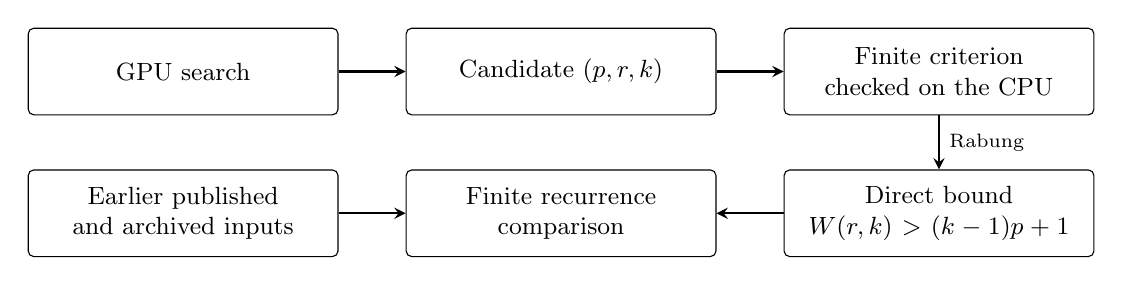
\begin{tikzpicture}[>=stealth,box/.style={draw,rounded corners=2pt,
  align=center,font=\small,minimum height=11mm,text width=3.7cm},
  edge/.style={->,thick}]
\node[box] (search) at (0,0) {GPU search};
\node[box] (triple) at (4.8,0) {Candidate $(p,r,k)$};
\node[box] (check) at (9.6,0) {Finite criterion\\checked on the CPU};
\node[box] (prior) at (0,-1.8) {Earlier published\\and archived inputs};
\node[box] (closure) at (4.8,-1.8) {Finite recurrence\\comparison};
\node[box] (bound) at (9.6,-1.8) {Direct bound\\$W(r,k)>(k-1)p+1$};
\draw[edge] (search)--(triple);
\draw[edge] (triple)--(check);
\draw[edge] (check)--node[right,font=\scriptsize]{Rabung}(bound);
\draw[edge] (bound)--(closure);
\draw[edge] (prior)--(closure);
\end{tikzpicture}
\caption{The two steps after discovery. The candidate can be checked without
replaying the search, and its bound is compared with consequences of earlier
inputs. Campaign coverage and the empirical intensity analysis are separate
from these pointwise implications.}
\label{fig:evidence-flow}
\end{figure}
